\begin{figure}
    \centering
    \begin{subfigure}{0.492\columnwidth}
        \centering
        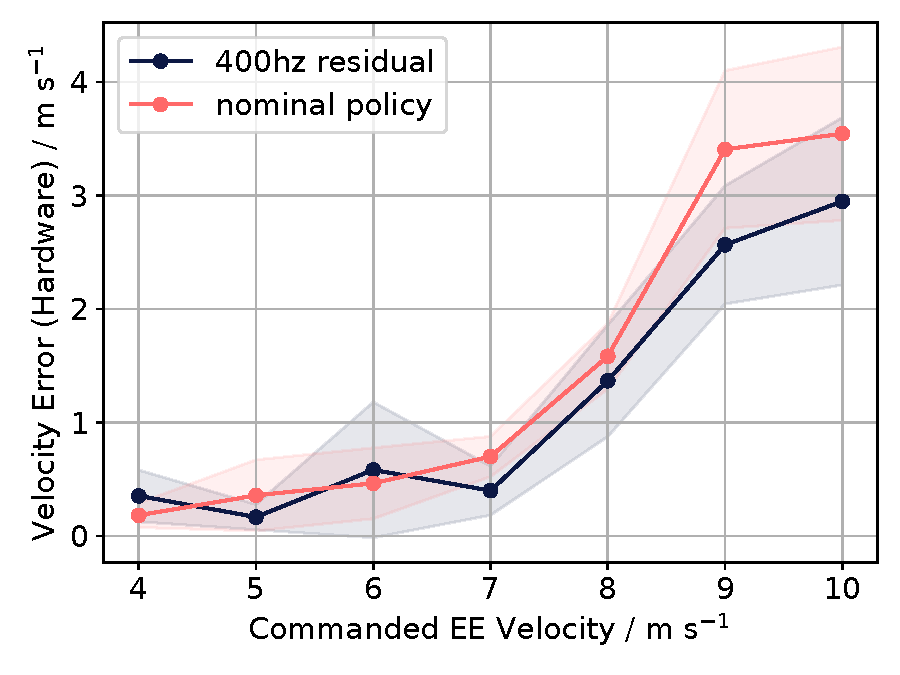
\includegraphics[width=\textwidth]{figures/swing_hw/swing_hw1.pdf}
        \caption{}
        \label{fig:swing_hw}
    \end{subfigure}
    \begin{subfigure}{0.492\columnwidth}
        \centering
        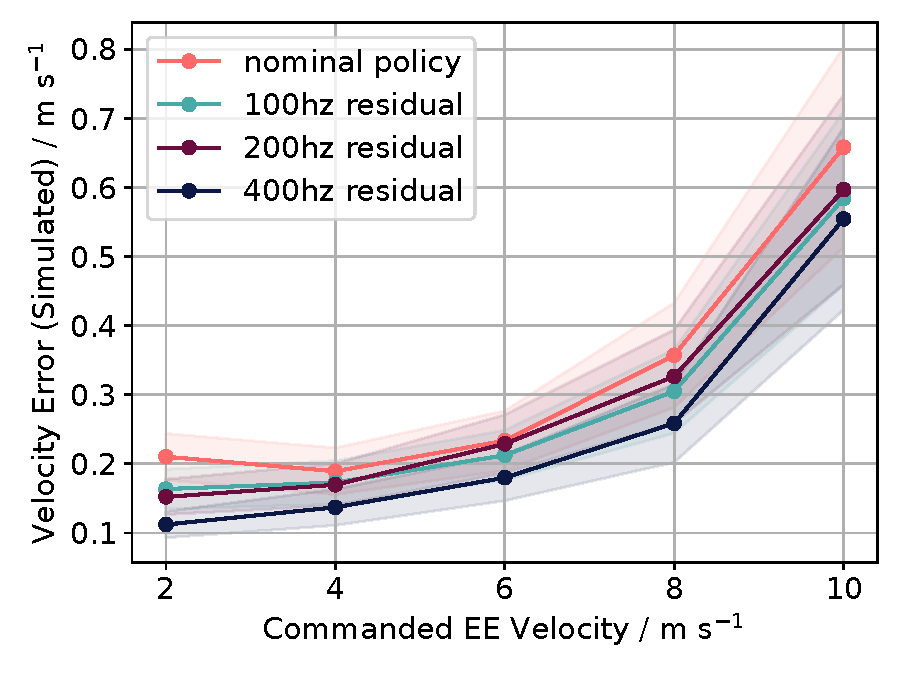
\includegraphics[width=\textwidth]{figures/swing_sim/swing_sim1.pdf}
        \caption{}
        \label{fig:swing_sim}
    \end{subfigure}
    \caption{\textbf{Comparison of residual policy effects in hardware and simulation.} 
    (a) EE velocity tracking improvement on hardware with the residual policy. The residual policy enhances tracking, especially at higher commanded end-effector velocities. 
    (b) Effectiveness of residual policies with various frequencies in simulation. All tested frequencies improve tracking over the baseline, with the 400 Hz residual policy achieving the best performance.}
    \label{fig:swing_combined}
\end{figure}
